
%(BEGIN_QUESTION)
% Copyright 2012, Tony R. Kuphaldt, released under the Creative Commons Attribution License (v 1.0)
% This means you may do almost anything with this work of mine, so long as you give me proper credit

Determine how to connect this DAQ unit to measure the output voltage of the Wheatstone bridge in such a way that an increasing compression on the strain gauge causes a {\it positive} indication at channel 3 of the DAQ, and that the same DAQ channel will register zero when the strain gauge is at rest:

$$\includegraphics[width=15.5cm]{i02121x01.eps}$$

\underbar{file i02121}
%(END_QUESTION)





%(BEGIN_ANSWER)

Remember that {\it stretching} a strain gauge causes its resistance to increase, while {\it compressing} a strain gauge causes its resistance to decrease: 

$$\includegraphics[width=15.5cm]{i02121x02.eps}$$

The two resistors (typically high-value, in the hundreds of kilo-ohms or even mega-ohms) provide a path for the DAQ's input bias currents, which is essential for a differential-input amplifier such as the instrumentation amplifier circuits inside the DAQ.

%(END_ANSWER)





%(BEGIN_NOTES)


%INDEX% Pictorial circuit review (analog signal wiring to data acquisition unit)

%(END_NOTES)


